%第3章


\section{詳細設計}

オブジェクト間のメッセージのやりとりを時系列に沿って表現するために,シーケンス図を作成した.以下にICタグを用いた商品識別システムのシーケンス図として,図\ref{sequence_ic}を載せる.

\begin{figure}[htbp]
\centering
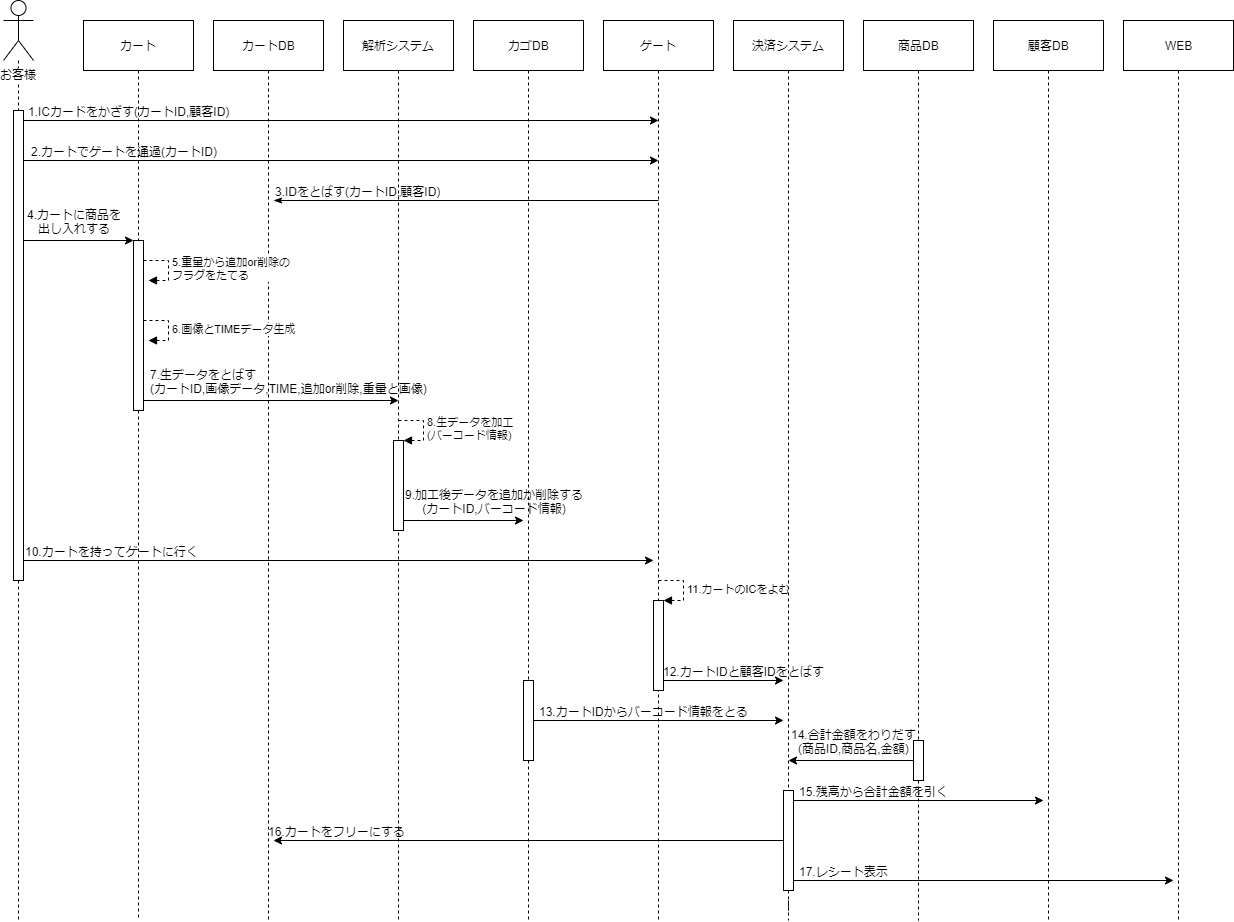
\includegraphics[width=15cm]{./picture/sequence_ic.eps}
\caption{ICタグを用いたシステムのシーケンス図}
\label{sequence_ic}
\end{figure}


図\ref{sequence_qr}はQRコードを用いたシステムのシーケンス図である.


\begin{figure}[htbp]
\centering
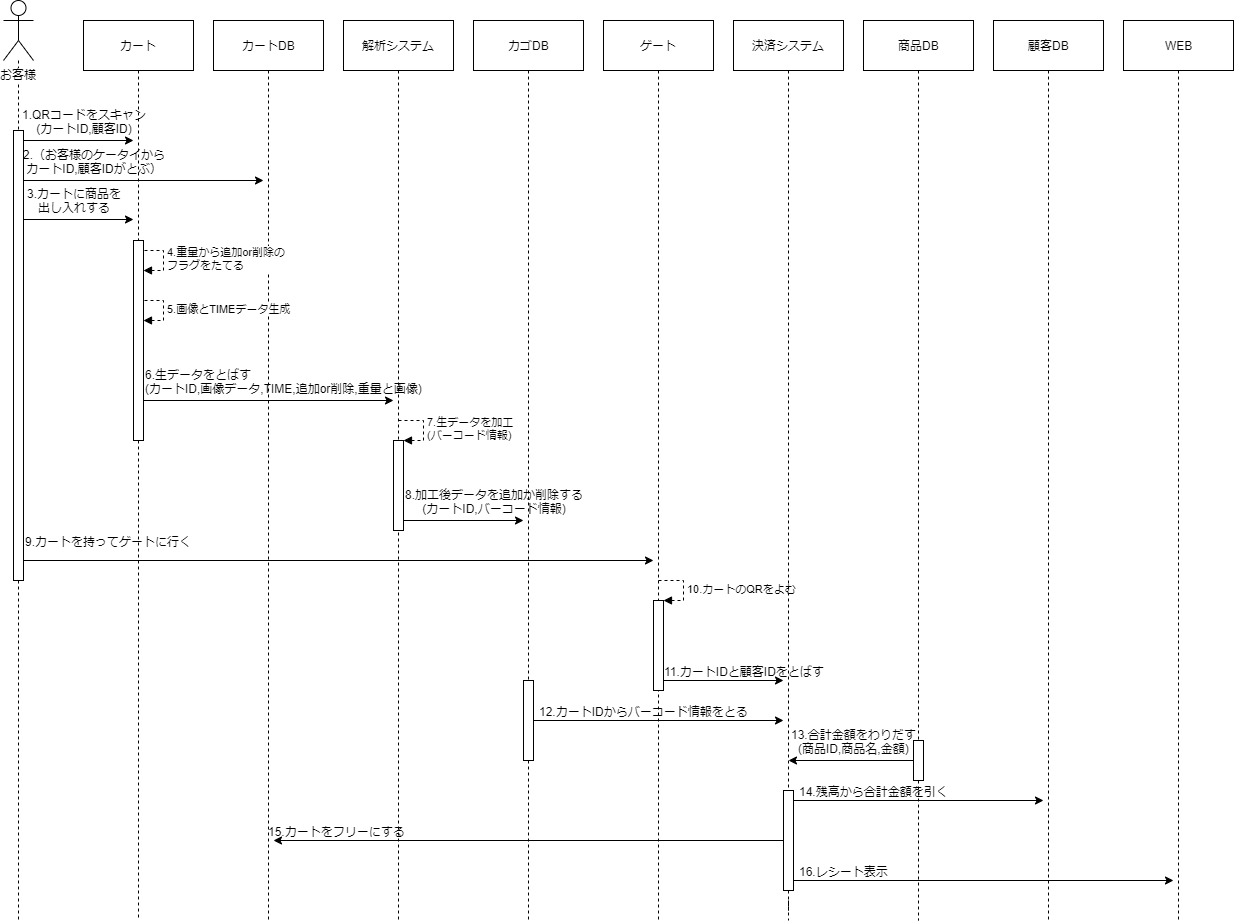
\includegraphics[width=15cm]{./picture/sequence_qr.eps}
\caption{QRコードを用いたシステムのシーケンス図}
\label{sequence_qr}
\end{figure}


図\ref{sequence_ic}と図\ref{sequence_qr}の違いはユーザ情報の登録の部分のみである.詳細設計まで行ったが,ICタグを用いたシステムとQRコードを用いたシステムの評価は3.2節から大きく変化しなかった.買い物と決済の設計においては共通しているため,そのまま優先度の高いシステムである下記の図\ref{sequence}部分を実装する.



\begin{figure}[htbp]
\centering
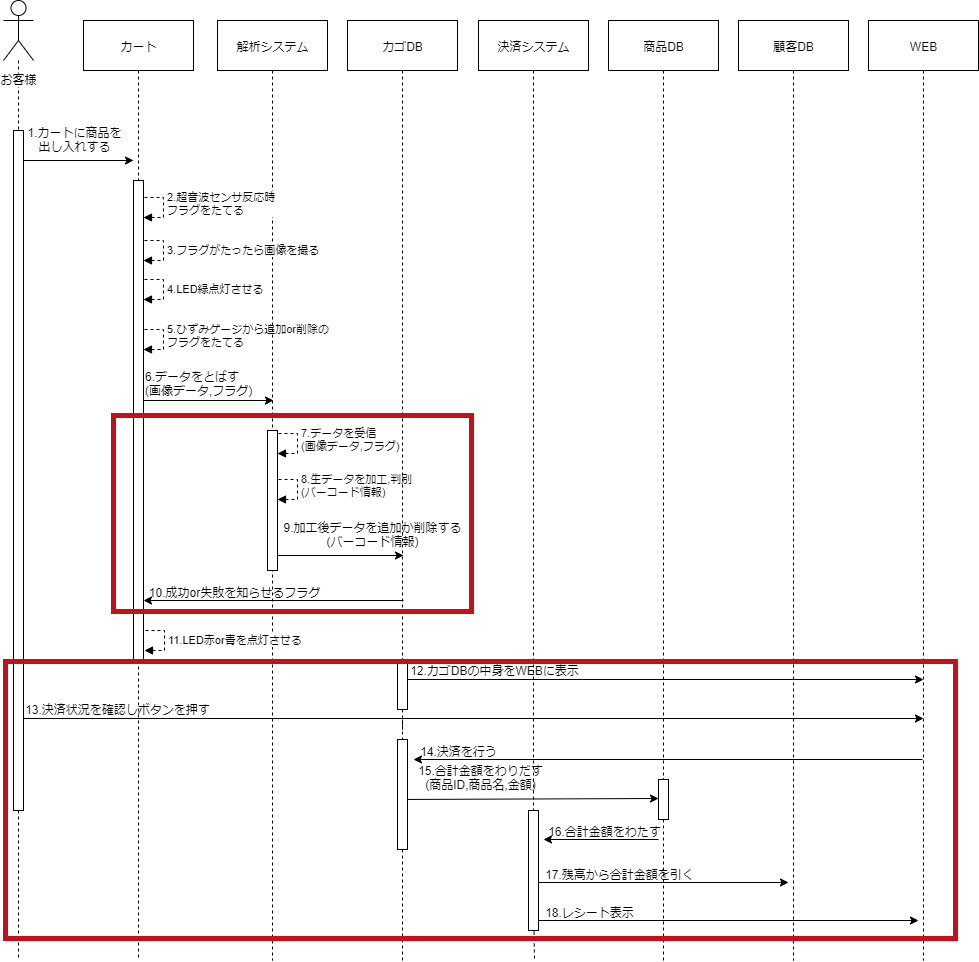
\includegraphics[width=15cm]{./picture/sequence.eps}
\caption{高優先度のシステムのシーケンス図}
\label{sequence}
\end{figure}


図\ref{sequence}において筆者の担当した部分はメッセージ2~6,10,11の部分である.各メッセージの詳細を下記に示す.


\begin{quote}
2. 超音波センサ反応時にフラグをたてる.

3. フラグがたったら,0.5秒に一度,合計6枚の画像を撮り,データ送信用配列にデータを追加する.

4. 画像を撮ったことをユーザに知らせるためにLED緑を点灯させる.

5. ロードセルより重量が増加したか減少したかを確認し,増加の場合は追加として1,減少の場合は削除として2のフラグをたて,キューへフラグを追加する.ただし,±3gの増減は誤差とする.

6. 追加,削除のフラグが入っているキューを参照し,データ送信用配列にフラグ情報を追加し,画像データと合わせてサーバへ送信する.

10. バーコード情報を正しく読み取れたか,読み取れなかったかを知らせるフラグをサーバから受信する.

11. サーバがバーコード情報を正しく読み取ることができた場合はLED青を,正しく読み取ることができなかった場合はユーザに再度商品の追加,削除を促すためLED赤を点灯させる.
\end{quote}

なお,優先度の高い項目部分において,単体テストの際に用いる,各センサのテスト項目を下記の表\ref{webcamera},表\ref{chouonpa},表\ref{rodoseru},表\ref{data}に示す.

\begin{table}[htbp]
\centering
\caption{Webカメラの単体テスト項目}
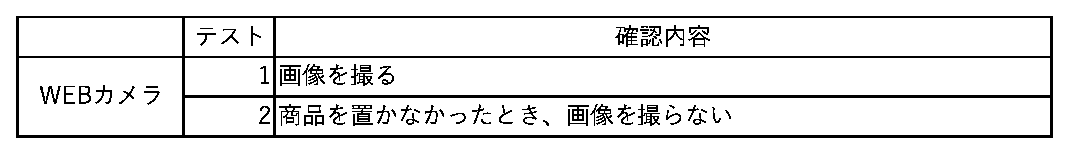
\includegraphics[width = 15cm]{./picture/webcamera.eps}
\label{webcamera}
\end{table}

\begin{table}[htbp]
\centering
\caption{超音波センサの単体テスト項目}
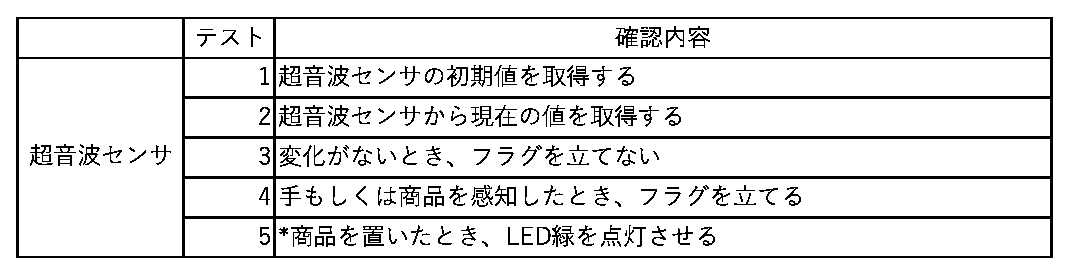
\includegraphics[width = 15cm]{./picture/chouonpa.eps}
\label{chouonpa}
\end{table}

\begin{table}[htbp]
\centering
\caption{ロードセルの単体テスト項目}
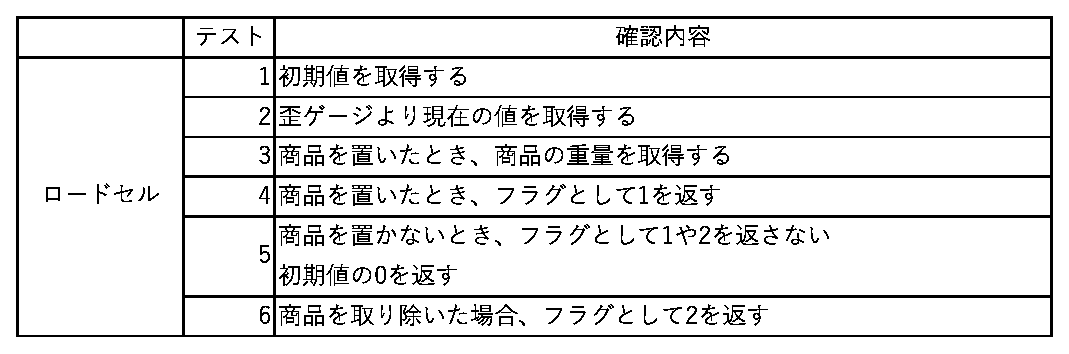
\includegraphics[width = 15cm]{./picture/rodoseru.eps}
\label{rodoseru}
\end{table}

\begin{table}[htbp]
\centering
\caption{データ送信の単体テスト項目}
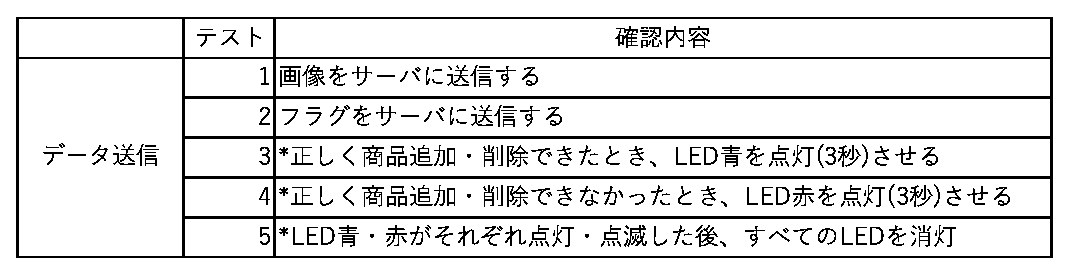
\includegraphics[width = 15cm]{./picture/data.eps}
\label{data}
\end{table}.


%メッセージの説明